% Options for packages loaded elsewhere
\PassOptionsToPackage{unicode}{hyperref}
\PassOptionsToPackage{hyphens}{url}
\PassOptionsToPackage{dvipsnames,svgnames,x11names}{xcolor}
%
\documentclass[
  10,
  a4paper,
]{article}

\usepackage{amsmath,amssymb}
\usepackage{lmodern}
\usepackage{iftex}
\ifPDFTeX
  \usepackage[T1]{fontenc}
  \usepackage[utf8]{inputenc}
  \usepackage{textcomp} % provide euro and other symbols
\else % if luatex or xetex
  \usepackage{unicode-math}
  \defaultfontfeatures{Scale=MatchLowercase}
  \defaultfontfeatures[\rmfamily]{Ligatures=TeX,Scale=1}
\fi
% Use upquote if available, for straight quotes in verbatim environments
\IfFileExists{upquote.sty}{\usepackage{upquote}}{}
\IfFileExists{microtype.sty}{% use microtype if available
  \usepackage[]{microtype}
  \UseMicrotypeSet[protrusion]{basicmath} % disable protrusion for tt fonts
}{}
\makeatletter
\@ifundefined{KOMAClassName}{% if non-KOMA class
  \IfFileExists{parskip.sty}{%
    \usepackage{parskip}
  }{% else
    \setlength{\parindent}{0pt}
    \setlength{\parskip}{6pt plus 2pt minus 1pt}}
}{% if KOMA class
  \KOMAoptions{parskip=half}}
\makeatother
\usepackage{xcolor}
\usepackage[lmargin=2cm,rmargin=2cm]{geometry}
\setlength{\emergencystretch}{3em} % prevent overfull lines
\setcounter{secnumdepth}{-\maxdimen} % remove section numbering
% Make \paragraph and \subparagraph free-standing
\ifx\paragraph\undefined\else
  \let\oldparagraph\paragraph
  \renewcommand{\paragraph}[1]{\oldparagraph{#1}\mbox{}}
\fi
\ifx\subparagraph\undefined\else
  \let\oldsubparagraph\subparagraph
  \renewcommand{\subparagraph}[1]{\oldsubparagraph{#1}\mbox{}}
\fi


\providecommand{\tightlist}{%
  \setlength{\itemsep}{0pt}\setlength{\parskip}{0pt}}\usepackage{longtable,booktabs,array}
\usepackage{calc} % for calculating minipage widths
% Correct order of tables after \paragraph or \subparagraph
\usepackage{etoolbox}
\makeatletter
\patchcmd\longtable{\par}{\if@noskipsec\mbox{}\fi\par}{}{}
\makeatother
% Allow footnotes in longtable head/foot
\IfFileExists{footnotehyper.sty}{\usepackage{footnotehyper}}{\usepackage{footnote}}
\makesavenoteenv{longtable}
\usepackage{graphicx}
\makeatletter
\def\maxwidth{\ifdim\Gin@nat@width>\linewidth\linewidth\else\Gin@nat@width\fi}
\def\maxheight{\ifdim\Gin@nat@height>\textheight\textheight\else\Gin@nat@height\fi}
\makeatother
% Scale images if necessary, so that they will not overflow the page
% margins by default, and it is still possible to overwrite the defaults
% using explicit options in \includegraphics[width, height, ...]{}
\setkeys{Gin}{width=\maxwidth,height=\maxheight,keepaspectratio}
% Set default figure placement to htbp
\makeatletter
\def\fps@figure{htbp}
\makeatother
\newlength{\cslhangindent}
\setlength{\cslhangindent}{1.5em}
\newlength{\csllabelwidth}
\setlength{\csllabelwidth}{3em}
\newlength{\cslentryspacingunit} % times entry-spacing
\setlength{\cslentryspacingunit}{\parskip}
\newenvironment{CSLReferences}[2] % #1 hanging-ident, #2 entry spacing
 {% don't indent paragraphs
  \setlength{\parindent}{0pt}
  % turn on hanging indent if param 1 is 1
  \ifodd #1
  \let\oldpar\par
  \def\par{\hangindent=\cslhangindent\oldpar}
  \fi
  % set entry spacing
  \setlength{\parskip}{#2\cslentryspacingunit}
 }%
 {}
\usepackage{calc}
\newcommand{\CSLBlock}[1]{#1\hfill\break}
\newcommand{\CSLLeftMargin}[1]{\parbox[t]{\csllabelwidth}{#1}}
\newcommand{\CSLRightInline}[1]{\parbox[t]{\linewidth - \csllabelwidth}{#1}\break}
\newcommand{\CSLIndent}[1]{\hspace{\cslhangindent}#1}

\makeatletter
\makeatother
\makeatletter
\makeatother
\makeatletter
\@ifpackageloaded{caption}{}{\usepackage{caption}}
\AtBeginDocument{%
\ifdefined\contentsname
  \renewcommand*\contentsname{Table of contents}
\else
  \newcommand\contentsname{Table of contents}
\fi
\ifdefined\listfigurename
  \renewcommand*\listfigurename{List of Figures}
\else
  \newcommand\listfigurename{List of Figures}
\fi
\ifdefined\listtablename
  \renewcommand*\listtablename{List of Tables}
\else
  \newcommand\listtablename{List of Tables}
\fi
\ifdefined\figurename
  \renewcommand*\figurename{Figure}
\else
  \newcommand\figurename{Figure}
\fi
\ifdefined\tablename
  \renewcommand*\tablename{Table}
\else
  \newcommand\tablename{Table}
\fi
}
\@ifpackageloaded{float}{}{\usepackage{float}}
\floatstyle{ruled}
\@ifundefined{c@chapter}{\newfloat{codelisting}{h}{lop}}{\newfloat{codelisting}{h}{lop}[chapter]}
\floatname{codelisting}{Listing}
\newcommand*\listoflistings{\listof{codelisting}{List of Listings}}
\makeatother
\makeatletter
\@ifpackageloaded{caption}{}{\usepackage{caption}}
\@ifpackageloaded{subcaption}{}{\usepackage{subcaption}}
\makeatother
\makeatletter
\@ifpackageloaded{tcolorbox}{}{\usepackage[many]{tcolorbox}}
\makeatother
\makeatletter
\@ifundefined{shadecolor}{\definecolor{shadecolor}{rgb}{.97, .97, .97}}
\makeatother
\makeatletter
\makeatother
\ifLuaTeX
  \usepackage{selnolig}  % disable illegal ligatures
\fi
\IfFileExists{bookmark.sty}{\usepackage{bookmark}}{\usepackage{hyperref}}
\IfFileExists{xurl.sty}{\usepackage{xurl}}{} % add URL line breaks if available
\urlstyle{same} % disable monospaced font for URLs
\hypersetup{
  pdftitle={Regional and Urban Economics},
  pdfauthor={Sindre Halvorsen Øveraas , Sebastian Mena Fløysand, Alen Colakovic \& Mona Lisa Jones},
  colorlinks=true,
  linkcolor={blue},
  filecolor={Maroon},
  citecolor={Blue},
  urlcolor={Blue},
  pdfcreator={LaTeX via pandoc}}

\title{Regional and Urban Economics}
\usepackage{etoolbox}
\makeatletter
\providecommand{\subtitle}[1]{% add subtitle to \maketitle
  \apptocmd{\@title}{\par {\large #1 \par}}{}{}
}
\makeatother
\subtitle{Dental industry}
\author{Sindre Halvorsen Øveraas , Sebastian Mena Fløysand, Alen
Colakovic \& Mona Lisa Jones}
\date{}

\begin{document}
\maketitle
\ifdefined\Shaded\renewenvironment{Shaded}{\begin{tcolorbox}[sharp corners, borderline west={3pt}{0pt}{shadecolor}, frame hidden, interior hidden, boxrule=0pt, enhanced, breakable]}{\end{tcolorbox}}\fi

\hypertarget{abstract}{%
\subsection{Abstract}\label{abstract}}

\texttt{The\ topic\ of\ research\ (What\ was\ studied)}

\texttt{The\ purpose\ (What\ was\ done)}

\texttt{The\ methodology\ (how\ the\ research\ was\ done)}

\texttt{Main\ findings\ (what\ was\ found)}

\texttt{Policy\ and\ implications\ (significance\ of\ findings)}

\hypertarget{introduction}{%
\subsection{Introduction}\label{introduction}}

Our main task in this assignment is to perform an analysis of geospatial
determinants of firm activity. More specifically we are to focus on the
Norwegian dental industry in this regard, and see how geospatial
determinants such as distances to shopping malls and CBDs (Central
Business Districts), as well as population density can determine dental
businesses income and general financial operations. As an example,
central questions in this assignment will be; ``Is it more beneficial to
be highly centralized in urban areas with high population density and
many competitors, or is it a greater advantage to be less centralized to
the advantage that the nearest competing company is considerably further
away?'', ``Which determinants appear to be most significant for economic
benefit?''

\texttt{A\ brief\ description\ of\ the\ problem\ and\ its\ importance}

\texttt{Statement\ of\ purpose\ or\ what\ was\ done}

\texttt{A\ brief\ description\ of\ main\ results}

\texttt{Description\ of\ methodology,\ main\ challenges\ and\ solutions}

\texttt{Discretion\ of\ the\ papers\ contribution\ in\ relation\ to\ previous\ research}

\texttt{Organization\ of\ paper}

\textbf{Hypothesis}

The location choice of firms providing service to end consumers,
significantly determine their ultimate growth potential.

\textbf{Research question}

What is the most profitable location for dental practice?

\hypertarget{theoretical-framework}{%
\subsection{Theoretical Framework}\label{theoretical-framework}}

Location theory gives regional economics its scientific disciplinary
identity and constitutes its theoretical methodological core
(\textbf{capello2011?}). It has typically microeconomic foundation and
uses theoretical models as well as adopting a statistical and
geographical approach (\textbf{capello2011?}). Furthermore, the theory
uses the concept of externalities in the spatial distribution of
activities, thereby laying the territorial bases for dynamic approach to
economic growth (\textbf{capello2011?}).

Regional growth theory involves spatial aspects of economic growth and
territorial distribution of income (\textbf{capello2011?}). It also
involves generating geographical advantages, in terms of easy or
difficult access to a particular area (\textbf{capello2011?}).

Furthermore, Keynesian economics emphasizes the importance of consumer
demand in driving economic growth. This may involve policies that
involve consumer spending, such as incentives for buying local products
or supporting small businesses or in this case preventing the the death
of down town due to competition from shopping malls. Subsequently,
increasing consumer demand, supporting business in a specific region.
Promoting economic growth or preventing economic decline
(\textbf{capello2016?}).

Harald Hotelling's locational equilibrium is determined by a logic of
profit maximization whereby each producer controls its own market area.
Productivity advantages of cities and urban clusters with a high density
of firms increase profit by attracting a larger number of potential
customers, and more productive workers (\textbf{capello2011?}).
Furthermore, the attractiveness of a central location increase the cost
of rent.

Alonso's bid rent model indicates the most profitable location for
firms. Closer to the centre with agglomeration attributes or in rural
areas with spacial monopoly and low rent. In gravitational models, the
attractiveness of the retail location, represent the size of the retail
centre. Furthermore, it depends on the variety of goods which can be
purchased at the same location (\textbf{mccann2013?}).

The model of potential has the capacity to measure the potential of
attractiveness to a place. Bigger cities or more heavily populated areas
have a stronger gravitational force. A possible indicator to predict
places of growth potential for dentist practice or shopping malls
(\textbf{capello2015?}).

\textbf{Interdependent location choice, the Hotelling's model (1929)}

The model assume that given the location of producers, and given demand
uniformly distributed geographically (in linear or circular form) the
market is divided into areas within each of which there operates a
single firm in a duopoly environment. Furthermore, no relocation costs
and demand only depend on location choice (\textbf{capello2015?}). The
location game starts off with the total market of AB, firm A in the
middle of location A and firm B starts in the middle of location B. One
firm starts relocating closer to the other to take some of the customers
in the other market area (\textbf{capello2015?}). The other respond by
doing the same and the game continues until both end up in the middle of
the market on the broader of AB. The end of the game is the position
where neither can increase sales volume by moving position
(\textbf{capello2015?}).

A simple explanation of why two dentists providing the same service, at
the same price might locate next to each other. Nevertheless, despite
increasing the transportation cost for patients. Perhaps the simplest
way to explain why there is a natural tendency for retailers to cluster
in space; a tendency which may help explain the existence of larger
agglomeration economies.

\textbf{Hotelling-Bertand model (1979)}

The Bertrand model was introduced as early as in 1883 and demonstrate
two firms competing by simultaneously setting prices for their
homogeneous products. Furthermore, the consumers choose the product with
the lowest price@tolotti2020. The model assumes that firms have
identical production cost and consumers have perfect information about
prices (\textbf{tolotti2020?}).

By combining elements from the two models a hybrid model of spatial
completion was birthed by Salop in 1979 (\textbf{tolotti2020?}). In this
model firms compete both in location and price, with consumers having a
transportation cost and firms producing differentiated products
(\textbf{tolotti2020?}).

\textbf{Marshall's agglomeration principles}

Marshall (1920) broadly divides externalities within agglomeration in
three main categories potentially drive sales. Firstly, knowledge
spill-over within industries or product specific technological
knowledge. Furthermore, market transactions in terms of value chain
transactions with industry-specialized buyers and suppliers. Lastly,
competition for specialized production factors such as labour and
product market competition (\textbf{nielsen2021?}).

There are solidly established conclusions regarding the existence of
agglomeration economies (\textbf{puga2010?}). However, less proof of
their estimated magnitude. Hence, identifying the causes of
agglomeration economies, is proving more difficult (\textbf{puga2010?}).
Nevertheless, there is a large theoretical literature that develops
these mechanisms (\textbf{puga2010?}). (\textbf{duranton2004?}) discuss
these classifications and identify \emph{learning, sharing} and
\emph{matching} as the main causes of agglomeration economies.

A larger market allows for a more efficient sharing of local
infrastructure and facilities. Therefore, a variety of intermediate
input suppliers, or a pool of workers with similar skills
(\textbf{puga2010?}). Despite higher rent the dental industry and
shopping malls, seams to reap higher benefits in more populated areas as
they are dependent on being located where there is a higher volume of
patients in order to drive sales. The attraction for the consumers and
users of public facilities is overall cost reduction
(\textbf{puga2010?}). Hence, the larger the population sharing
facilities the lower the cost per user (\textbf{puga2010?}). Presumably,
industrial factories and business clusters are more dependent on being
close to raw materials and industrial action.

Furthermore, a larger market also allows for a better matching between
employers and employees, improved chances of finding suitable and better
quality of matches (\textbf{puga2010?}). Shopping malls require skilled
workers to drive sales. However, they are not so dependent on highly
educated workers as dentists whom according to resent study, tend to
prefer bigger cities (as they are highly educated)
(\textbf{davis2020?}). More-so, cites provide a constant market for
specialized skills and more productive work force (\textbf{puga2010P?})
Perhaps, a possibility for higher wages being compensated by more
efficient workers in bigger agglomeration economies. That said the
Norwegian cities might differ from the american cites in the study, as
the population and clusters are no where near the same size. Lastly, a
larger market can also facilitate learning by promoting the development
and widespread adaptation of new technologies and business practice
(\textbf{puga2010?}).

Interactions with experienced workers helps acquire valuable skills.
Experienced workers remain in cities to share the rent of this learning
process (\textbf{puga2010?}). Besides this purposeful transition of
knowledge, the information literature on learning in cities has also
emphasized the unintended casual flow of information facilitated by big
cities.'' (\textbf{puga2010?})

\textbf{Urban location of dentist; The Alonso model}

The Alsonso model demonstrate geographical locations tied up to
location. Furthermore, It is an urbanized formulation of the nineteenth
century von Thünen model (\textbf{capello2015?}). In this case used to
get an indicating of where the most profitable location for dental
practise.

Alonso assumes the existence of a city that cannot be build
instantaneously, and therefore of an effective rent-curve from the city
centre to the periphery. Furthermore, it determines the location for a
new firm willing to locate in the city and the profit the firm can
obtain. In some cases different from the normal or average price
competition (\textbf{capello2015?}).

As the Von Thünen assume a uniformed space where all land is equally
fertile, this model envisages a city, endowed with infrastructure which
cover the entire city in all directions whereas unit transport costs are
constant in space. More-so, the town or city has a single centre point.
The city centre of business district (CBD) is generally defined as the
most attractive for all firms. (\textbf{capello2015?}). The model also
assume perfect competition and unlimited demand, in other words it is
supply-orientated (\textbf{capello2015?}). Furthermore, demonstrating a
specific production function with fixed coefficients and constant
returns to scale.

Rent obtained in the model is the remainder left after transport,
production costs and profit has been subtracted from revenues
(\textbf{capello2015?}). The bid-rent curve will in this case
demonstrate the prise of rent within Bank and Financial locations,
Retail locations, and industrial locations.

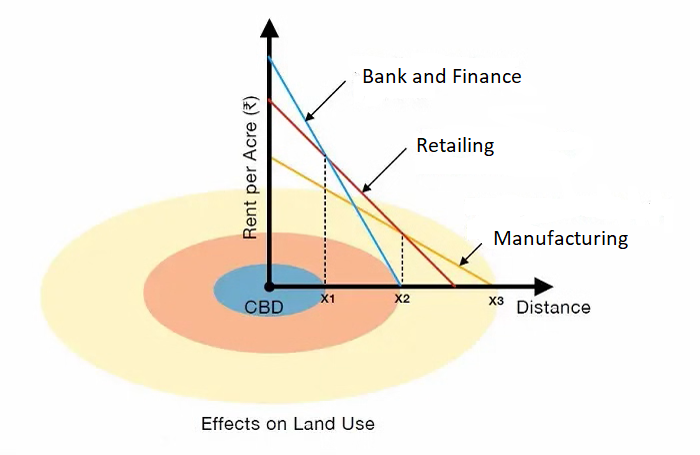
\includegraphics{images/bidrent.gpg.jpg}

The illustration shows three categories: The most expensive rent closest
to the centre is the Bank and finance district, followed by the retail
agglomeration areas and industrial sites furthest away from the central
point. Dental practices are service orientated thus depending on
population density and central activities. Opening hours are relay
outside of office hours. Production cost does not appear to be important
in this case since dentist is a public service. Hence, not dependent of
regular transportation of sales goods. The rent realized by the
landowner is the envelope of the three rent supply curves
(\textbf{capello2015?}).

From a Marshallian way of thinking dentists should cluster somewhere in
this pink area to reap maximum sales volume. Furthermore, they may also
increase their profits further out in to other retail agglomeration
area. The attractiveness might be high in these places due to economies
of scope. As the positive benefits from the Marshallian agglomeration
attributes play out. Subsequently, increasing profit by trading higher
transportation cost for lower rent. In addition fewer dentists to
compete with supporting the hotellings game theory whereas companies
more to achieve spatial monopoly (\textbf{mccann2013McCann?}).

\textbf{Gravitational models}

The centre attracts firms, people and activities. Furthermore, it
influence the central points in diverse ways such as commuter movements,
diffusion of knowledge, corporations and network and personal
relationship (\textbf{capello2015?}). More-so, they are generated by the
intensity of the flows generated between places (\textbf{capello2015?}).
The gravitational pull to a place of interest for a dentist will
determine how much sales can be generated by locating there. Several
locations can then be measures against each other to determine profit
maximisation.

These models has the potential to measures the future attractiveness of
a place. Changes in infrastructure such as easier access to a place
might change the attractiveness of a place or move the flow of people.
Subserviently, increasing the gravitationally pull between the two
places. Furthermore, The model uses population and distance to measure
the attractiveness and relations between two places
(\textbf{capello2015?}). Furthermore, these models have predictive
capacity and can be used to estimate the potential impact. In
particular, location of new productive activity in an area
(\textbf{capello2015?}). For instance predict where to build a shopping
centre (\textbf{capello2015?}). By taking these factors in to account
dentist could predict the most profitable locations in years to come by
predicting the amount of people that will move from one city to another
or tow different points of interest within a city.

\textbf{Retail Agglomeration and Economies of Shopping Centres}

Town and cities have long had shopping districts in which stores are
concentrated. To some extent such centre points were the result of
uncoordinated store-location decisions (\textbf{brueckner2011?}).
Nevertheless, not coincidentally according to Hotelling's theory (1929).
He describes the concentration of retail stores by a market desire to
create a Nash equilibrium. At this point all retailers expected sales
maximisation outcome cannot be improved by changing position.
Contradictory to the assumption that consumers will shop at the nearest
retailer, they are willing to travel significantly further to reach
certain central places. Marshall (1920) points out another explanation
for this in his seminal work on agglomeration. That being,intra-industry
knowledge spillovers as mechanisms leading to formation of industry
cluster (\textbf{nielsen2021?}). In this case the dental industry
information spillovers are bounded in geographical space. Hence, the
need to locate in close proximity. That being the latest equipment, in
order to work faster or the right personnel to attract more patients.
Another way to drive sales in this area could be by dentist
specialisation and patients referrals between dentists.

Another important externalities expressed in Marshall (1920) theory is
market transactions. Whereas, geographical proximity reduces transaction
cost through several mechanism (\textbf{nielsen2021?}). The market
transactions can be extended to the endogenous location of specialized
human capital (\textbf{nielsen2021?}). ``It is well known among
economists and other social scientists that large cities have
disproportionately large shares of highly educated workers, and the
trend has been growing in recent decades.'' (\textbf{bakerBaker?}).
Presumably, larger cities would then be more attractive to dentists in
terms of cost and quality of specialised labour in smaller towns.
Especially, those trying to achieve spatial monopoly end up loosing
profit by overpaying for labour or in worst case scenario not finding
enough dentists labour and end up compromising on quality. In both cases
growth potential would be compromised.

Marshall also points out the competition within the geographical
location. Hence, the marketplace and business districts give consumers
low search and switching costs (\textbf{capello2015?}). The fact that
owners of stores seem to prefer highly concentrated shopping. More-so,
it suggests that the sales volumes outweigh the loss attributed to
greater price competition@capello2015.

\textbf{Shopping Malls}

Owners of shopping malls ``orchestrate'' the process of retail
agglomeration that happens naturally in towns and cities
(\textbf{brueckner2011?}). Naturally, the same retail agglomeration and
Nash equilibrium may occur in shopping malls if not more intensely as
the shops are in closer proximity. Furthermore, the potential for more
knowledge spillovers, higher volume of market transaction and more
competition. When retail agglomeration is orchestrated by the owner of a
shopping mall, the strength and direction of such externalities are
taken into account (\textbf{brueckner2011?}). Much so, because the price
of rent is dependent on the overall revenue of a shopping mall. Hence,
the owner of the mall wants to choose the mix of stores and their sizes
taking these externalities, attributes and anchor stores attractiveness
into account (\textbf{brueckner2011?}).

The Norwegian retail market for alcoholic beverages is controlled by the
state monopoly. Anchor-stores such as the Wine-monopoly bring in a
higher volume of consumers (\textbf{lai2013Lai?}). For example, shoppers
visiting the Wine-monopoly in a mall may also visit a clothing store,
and even find it beneficial to use public services at the same time.
Nevertheless, they are limited in numbers and needs government approval.
Each municipality must apply to get the wine monopoly in their area. One
of the factors considered in this process is the death of city centre. A
possible reason for this is so called ``predatory malls'' which are
purposely built to overtake the exciting local market. Perhaps more so
if malls cater for cinema, restaurants, bars and other attributes in
conjunction with the city centre. Not to mention the upper hand of easy
road access and free parking.

\hypertarget{data}{%
\subsection{Data}\label{data}}

\texttt{In\ quantitative\ studies\ this\ section\ provides\ details\ about\ dataset,\ variables,\ instruments\ and\ measurement\ procedures\ used\ in\ the\ study.\ If\ the\ data\ was\ collected\ by\ the\ authors\ this\ section\ will\ describe\ how\ the\ sample\ was\ collected.\ If\ specific\ instruments\ were\ constructed\ to\ collect\ the\ data\ they\ will\ be\ described\ here\ and\ included\ in\ the\ appendix.\ Procedures\ used\ to\ measure\ variables\ are\ often\ described\ in\ sufficient\ detail\ to\ permit\ replication.\ In\ economic\ papers,\ this\ section\ describes\ the\ empirical\ model\ and\ estimation\ strategy\ used\ by\ the\ authors.}

\textbf{Data description}

(Data and how it was collected)

\textbf{Empirical Specification}

Included why and why not outliner????

\textbf{Estimation strategy}

\textbf{Analytical framework}

SEDA (Spatial Explanatory Data Analyses)

Spatial data analysis is a rapidly growing area in Statistics
(\textbf{haslett1992?}). The Journal of the statistics society define
such data as being objects in space, which objects have physical
location. Furthermore, the analyses are spatial if these locations are
relevant to the interpretation of the data (\textbf{haining1998?}).

The examination of the data involves the examination of data collected
from q-gis maps;
\texttt{it\ will\ involve\ little\ more.\ Graphical\ techniques\ for\ examining\ such\ maps\ are\ thus\ a\ central\ part\ of\ the\ methodology.\ A\ number\ of\ such\ techniques\ are\ discussed."}
(\textbf{haslett1992?}).

\texttt{What\ data\ are\ used?}

\texttt{What\ has\ been\ calculated?}

\hypertarget{econometric-approach}{%
\subsection{\texorpdfstring{\textbf{Econometric
Approach}}{Econometric Approach}}\label{econometric-approach}}

The questions addressed are related to the geographical space of Norway.
Norway is a country with relatively small population and large
heterogeneous land area. Furthermore, the population is decentralized
with the majority of population living in urban areas. This unique
spatial distribution of land might give a possible explanation to
diversions from the simple theoretical models used in this paper.
Whereas one of the assumptions are homogeneous landscape. Nevertheless,
the way economies are organised comes partly from the emergence of
centralities within a city. Transportation networks have the potential
to increase sprawl depending on how the urban system evolves gradually.

The results from the bid rent configuration from the city centre gave
the opportunity to explore other locations in each municipality's.
Having an urban system of multiple centres and applying the same logic
of the model to other retail agglomeration areas. Resulting in finding
relationships based on three different types of distance measurements.
Firstly, the distance between Dental Practice and CBD then, dentist and
other retail agglomeration areas and lastly amongst dentists. Finding
that most dentist are either located close to a City, Central Business
District or a shopping mall. Additionally, dentist also located close to
each other making some sort of industrial cluster. Supporting,
Marshall's agglomeration theory on knowledge spillovers, increasing the
sills to attract more patients.

Furthermore, when using the dentist income (y) and comparing the
distance from the mall (x), signs of patterns emerge showing that income
is greater when the dentist is placed closer to the shopping mall.
Furthermore, decreasing as the distance gets bigger. Faster
transportation can increase convenience of commuting, increasing rent
commuters from the city centre are willing to pay, and therefore
increasing the area of developed land without this being necessary
corresponding to an increase in population. Hence supporting findings;
when the distance reach around 10km from the mall the income starts to
increase before it decrease again around 20km. Also in line with the
Keynesian theory suggesting that this pattern might take place as the
transportation cost for individuals further away from the Shopping mall
does not increase to much by travelling the extra distance. Hotelling
also describes this case where the consumer are willing to travel
further to reach a certain central place.

According to the Alons's model dentist should locate in the retail area
for higher volume of sales. Dentist being placed further out in to other
retail agglomeration areas can also be a good strategy. However, the
dentist would then rely on the area having less competition so the rate
between competition and population density are proportional. Our
findings in QGIS shows that in areas of high population density, the
number of dentist also increase. The consumer/patient then has more to
choose between and the dentist also has a bigger scale of potential
customers. Where in smaller areas it is less competition and the dentist
would appear to have somewhat of a monopoly since the transportation
cost to the second closes dentist are noticeable higher.

Furthermore, being aware of the fact that going to the dentist is a
public services and most people get assigned to their closest dentist
based on their living address. This also takes away some of the
competition and would support placement in more rural areas. More-so, is
important to notice that when passed 18 years of age, you could risk
loosing your local public dentist due to lack of capacity. Suggesting
some dentist might seek closer to CBD areas to capture most of the
remaining part of the population. Business, public places and industry
can have a positive effect on revenue since this is areas where most of
the population spends their time during their day, either going to work,
school and other errand. Reducing the transportation cost for the
customer as they are already located in these areas even if they do not
live here.

The bid rent models are under the assumption that Dentists use spatial
completion to maximise profit. Nevertheless, the cost of dental care in
Norway can vary depending on a number of other factors such as the type
of treatment, the location of the dental practice and the dentist
experience and qualifications. The Norwegian Dental Association rate the
average cost of check ups is between four to eight hundred Norwegian
Krone's {``Tannlegeforeningen''} (n.d.). Bertrand model also take price
as competitive advantage in to consideration.

Viser data noe om indikasjon på dyrere priser i nærheten av større byer
of hvor det er stedsbestemt monopol? Tjener tannleger i større byer mer?
Her kan vi også skrive om gravitasjons modeller.

Another Mashiallian point to be made could be the advantage of industry
clusters. Taken for granted that the data on Dentist includes both
``normal Dentists'' and specialist. Where in this case a ``normal
dentist'' would for example recommend one of their customers to go see a
specialist to get braces. The customer would then probably prefer to go
to the closes specialist. The access to work force in these areas would
also be good and will be within the same geographic area.

Shopping malls have a relatively short history in Norway, with the first
shopping mall opening in the late sixties. Prior to the most retail
activities took place in the city centre. Furthermore, these malls
typically featured a mix of shops, restaurants and entertainment
options, and they were often located in suburban areas or on the
outskirts of cities {``Home - NCSC''} (n.d.). In resent years, there has
been a trend towards larger and more comprehensive shopping malls in
Norway {``Home - NCSC''} (n.d.).

However, the growth of shopping malls in Norway has not been without
controversy. Some critics argue that the development of large shopping
malls has led to the decline of traditional shopping streets and local
businesses, while other raise concerns about the environmental impact of
these large scale commercial developments {``Kan Vin Og Sprit Skape
Byutvikling?''} (2014).

Information about Wine monopoly locations has also been studied in this
paper. As the wine monopoly are anchor stores they may affect the
attractiveness of the shopping mall {``Kan Vin Og Sprit Skape
Byutvikling?''} (2014). The Norwegian government regulates the
placements of wine monopoly stores in shopping malls to prevent
completion with town centres omsorgsdepartementet (2022). More
importantly, the government may take in to account the potential impact
of exciting retail centres in the region. This regional economic
approach aim to promote sustainable development and balance economic
growth across the country {``Kan Vin Og Sprit Skape Byutvikling?''}
(2014).

Hva viser informasjonen om vinmonopolet?

\hypertarget{conclusion}{%
\subsection{Conclusion}\label{conclusion}}

\hypertarget{references}{%
\subsection*{References}\label{references}}
\addcontentsline{toc}{subsection}{References}

\hypertarget{refs}{}
\begin{CSLReferences}{1}{0}
\leavevmode\vadjust pre{\hypertarget{ref-home-n}{}}%
{``Home - NCSC.''} n.d.
\href{https://ncscnordic.org/,\%20https://ncscnordic.org/}{https://ncscnordic.org/,
https://ncscnordic.org/}.

\leavevmode\vadjust pre{\hypertarget{ref-kanvin2014}{}}%
{``Kan Vin Og Sprit Skape Byutvikling?''} 2014.
\url{https://www.aftenposten.no/kultur/i/oEy0/kan-vin-og-sprit-skape-byutvikling}.

\leavevmode\vadjust pre{\hypertarget{ref-omsorgsdepartementet2022}{}}%
omsorgsdepartementet, Helse-og. 2022. {``Vinmonopolordningen.''}
\emph{Regjeringen.no}. regjeringen.no.
\url{https://www.regjeringen.no/no/tema/helse-og-omsorg/psykisk-helse/innsikt/vinmonopolordningen/id2528183/}.

\leavevmode\vadjust pre{\hypertarget{ref-tannlege}{}}%
{``Tannlegeforeningen.''} n.d. \url{https://www.tannlegeforeningen.no/}.

\end{CSLReferences}



\end{document}
